% ============================================================================
% Multilingual ASR Pipeline --- Beamer Presentation (15 slides)
% ============================================================================
\documentclass[aspectratio=169, 11pt]{beamer}

% ── Theme & Colors ──────────────────────────────────────────────────────────
\usetheme{Madrid}
\usecolortheme{whale}

% Custom colors
\definecolor{pipeblue}{RGB}{41, 98, 168}
\definecolor{pipeteal}{RGB}{0, 150, 136}
\definecolor{pipeorange}{RGB}{230, 126, 34}
\definecolor{pipegray}{RGB}{100, 100, 100}
\definecolor{pipegreen}{RGB}{39, 174, 96}
\definecolor{pipered}{RGB}{192, 57, 43}
\definecolor{lightbg}{RGB}{245, 248, 252}

\setbeamercolor{structure}{fg=pipeblue}
\setbeamercolor{frametitle}{bg=pipeblue, fg=white}
\setbeamercolor{title}{bg=pipeblue, fg=white}
\setbeamercolor{block title}{bg=pipeblue, fg=white}
\setbeamercolor{block body}{bg=lightbg}
\setbeamercolor{block title alerted}{bg=pipeorange, fg=white}
\setbeamercolor{block body alerted}{bg=lightbg}
\setbeamercolor{block title example}{bg=pipegreen, fg=white}
\setbeamercolor{block body example}{bg=lightbg}

% ── Packages ────────────────────────────────────────────────────────────────
\usepackage{fontenc}
\usepackage{inputenc}
\usepackage{graphicx}
\usepackage{booktabs}
\usepackage{tikz}
\usepackage{xcolor}
\usepackage{listings}
\usepackage{fontawesome5}
\usepackage{multicol}
\usepackage{adjustbox}

\usetikzlibrary{shapes.geometric, arrows.meta, positioning, calc, fit, backgrounds, shadows}

% ── Listings style ──────────────────────────────────────────────────────────
\lstset{
    basicstyle=\ttfamily\scriptsize,
    backgroundcolor=\color{lightbg},
    frame=single,
    rulecolor=\color{pipeblue!30},
    breaklines=true,
    columns=fullflexible,
    keepspaces=true,
    showstringspaces=false,
}

% ── Footer ──────────────────────────────────────────────────────────────────
\setbeamertemplate{navigation symbols}{}
\setbeamertemplate{footline}{
    \leavevmode\hbox{%
        \begin{beamercolorbox}[wd=.333\paperwidth,ht=2.5ex,dp=1ex,center]{author in head/foot}%
            \usebeamerfont{author in head/foot}\insertshortauthor
        \end{beamercolorbox}%
        \begin{beamercolorbox}[wd=.334\paperwidth,ht=2.5ex,dp=1ex,center]{title in head/foot}%
            \usebeamerfont{title in head/foot}\insertshorttitle
        \end{beamercolorbox}%
        \begin{beamercolorbox}[wd=.333\paperwidth,ht=2.5ex,dp=1ex,right]{date in head/foot}%
            \usebeamerfont{date in head/foot}\insertframenumber{} / \inserttotalframenumber\hspace*{2em}
        \end{beamercolorbox}}%
    \vskip0pt%
}

% ── Title Info ──────────────────────────────────────────────────────────────
\title[ASR Pipeline]{Multilingual ASR Pipeline}
\subtitle{Automated Speech Transcription, Speaker Identification \& Translation}
\author{Sayouti Noureini}
\date{\today}
\institute{Work in Progress}

% ============================================================================
\begin{document}

% ── Slide 1: Title ─────────────────────────────────────────────────────────
\begin{frame}[plain]
    \titlepage
\end{frame}

% ── Slide 2: Outline ──────────────────────────────────────────────────────
\begin{frame}{Outline}
    \tableofcontents
\end{frame}

% ============================================================================
\section{Overview}
% ============================================================================

% ── Slide 3: What Does the Pipeline Do? ────────────────────────────────────
\begin{frame}{What Does the Pipeline Do?}
    \begin{columns}[T]
        \begin{column}{0.55\textwidth}
            \vspace{0.5em}
            Given an \textbf{audio recording} in \textbf{any language}, the pipeline automatically produces:
            \vspace{0.5em}
            \begin{itemize}
                \item[\faFileAlt] A \textbf{professional transcript}
                \item[\faUsers] \textbf{Speaker identification} --- who said what
                \item[\faClock] \textbf{Precise timestamps} for every utterance
                \item[\faLanguage] \textbf{English translation} of all content
                \item[\faMagic] \textbf{Cleaned-up text} --- ready for analysis
            \end{itemize}
            \vspace{0.8em}
            \begin{alertblock}{Key Strength}
                Supports \textbf{1,600+ languages}, including low-resource languages often ignored by commercial tools.
            \end{alertblock}
        \end{column}
        \begin{column}{0.42\textwidth}
            \centering
            \begin{tikzpicture}[
                box/.style={
                    rounded corners=4pt,
                    minimum width=4.5cm,
                    minimum height=0.8cm,
                    align=center,
                    font=\small\bfseries,
                    text=white,
                    drop shadow={shadow xshift=0.5mm, shadow yshift=-0.5mm}
                },
                arr/.style={-{Stealth[length=3mm]}, thick, pipeblue!70}
            ]
                \node[box, fill=pipeblue] (input) at (0,0) {\faMusic\ \ Audio File};
                \node[box, fill=pipeteal, below=0.5cm of input] (process) {\faCogs\ \ 7-Stage Pipeline};
                \node[box, fill=pipegreen, below=0.5cm of process] (output) {\faFileAlt\ \ Transcript};
                \draw[arr] (input) -- (process);
                \draw[arr] (process) -- (output);
                \node[font=\tiny\itshape, text=pipegray, right=0.1cm of input] {any format};
                \node[font=\tiny\itshape, text=pipegray, right=0.1cm of process] {fully automated};
                \node[font=\tiny\itshape, text=pipegray, right=0.1cm of output] {TXT / JSON / SRT};
            \end{tikzpicture}
        \end{column}
    \end{columns}
\end{frame}

% ============================================================================
\section{Hardware \& Performance}
% ============================================================================

% ── Slide 4: Hardware Specifications ───────────────────────────────────────
\begin{frame}{Hardware Specifications}
    \begin{columns}[T]
        \begin{column}{0.45\textwidth}
            \begin{block}{\faDesktop\ \ Development Machine}
                \small
                \renewcommand{\arraystretch}{1.2}
                \begin{tabular}{@{}l l@{}}
                    \faMemory\ \textbf{GPU} & NVIDIA --- \textbf{6\,GB VRAM} \\
                    \faMicrochip\ \textbf{CPU} & Multi-core \\
                    \faHdd\ \textbf{RAM} & 16\,GB system \\
                    \faLinux\ \textbf{OS} & WSL2 on Windows 11 \\
                    \faPython\ \textbf{Runtime} & Python 3.12 + CUDA \\
                \end{tabular}
            \end{block}
            \vspace{0.2em}
            \begin{alertblock}{\faExclamationTriangle\ \ The 6\,GB Constraint}
                \scriptsize
                Most ASR pipelines assume 16--24\,GB VRAM.
                With only \textbf{6\,GB}, every decision is driven by
                \textbf{memory efficiency}.
            \end{alertblock}
        \end{column}
        \begin{column}{0.52\textwidth}
            \begin{block}{\faCogs\ \ How the Pipeline Adapts}
                \scriptsize
                \begin{itemize}
                    \item[\faBolt] \textbf{Sequential model loading} --- one model on GPU at a time
                    \item[\faTrashAlt] \textbf{Explicit unloading} --- \texttt{load()/unload()} lifecycle
                    \item[\faCompressArrowsAlt] \textbf{4-bit quantization} --- TranslateGemma 4B in $\sim$2.5\,GB
                    \item[\faLayerGroup] \textbf{GPU memory flush} --- \texttt{empty\_cache()} + \texttt{gc.collect()}
                    \item[\faRulerHorizontal] \textbf{float16 compute} --- halves memory vs.\ float32
                    \item[\faCubes] \textbf{CTC 300M} over 1B --- fits in 6\,GB with room to spare
                \end{itemize}
            \end{block}
        \end{column}
    \end{columns}
\end{frame}

% ── Slide 5: Performance ──────────────────────────────────────────────────
\begin{frame}{Performance on 6\,GB GPU}
    \begin{columns}[T]
        \begin{column}{0.48\textwidth}
            \begin{exampleblock}{\faStopwatch\ \ Current Benchmark}
                \centering
                \vspace{0.3em}
                {\Large\bfseries 8 minutes} processing time\\[3pt]
                for a \textbf{20-minute} audio file\\[4pt]
                \colorbox{pipegreen!15}{\parbox{0.8\linewidth}{\centering
                    \small Real-Time Factor: \textbf{0.4$\times$}\\[-1pt]
                    \scriptsize(faster than real-time)
                }}
                \vspace{0.3em}
            \end{exampleblock}
            \vspace{0.2em}
            \begin{block}{\faFlask\ \ Real Test (Spanish, 20 min)}
                \scriptsize
                \renewcommand{\arraystretch}{1.1}
                \begin{tabular}{@{}l l@{}}
                    \textbf{Engine} & Whisper large-v3 \\
                    \textbf{Speakers} & 5 identified \\
                    \textbf{Speech} & 61\% speech, 39\% non-speech \\
                    \textbf{Translation} & TranslateGemma \\
                    \textbf{Time} & \textbf{8 min} end-to-end \\
                \end{tabular}
            \end{block}
        \end{column}
        \begin{column}{0.48\textwidth}
            \begin{block}{\faRocket\ \ Speed Optimizations}
                \scriptsize
                \begin{enumerate}
                    \item \textbf{Parallel execution} --- transcription \& diarization run concurrently
                    \item \textbf{Batched inference} --- Whisper batched pipeline (batch\_size=8)
                    \item \textbf{VAD-guided chunking} --- skips silence, only processes speech
                    \item \textbf{Lazy model loading} --- models load on first use
                    \item \textbf{Spectral noise reduction} --- cleaner audio = faster ASR
                \end{enumerate}
            \end{block}
            \vspace{0.2em}
            \begin{alertblock}{\scriptsize\faMemory\ \ Memory Choreography}
                \scriptsize
                ASR models unloaded \textit{before} translation loads.
                Peak VRAM never exceeds $\sim$4\,GB at any stage.
            \end{alertblock}
        \end{column}
    \end{columns}
\end{frame}

% ============================================================================
\section{Pipeline Architecture}
% ============================================================================

% ── Slide 6: The 7-Stage Pipeline ─────────────────────────────────────────
\begin{frame}{The 7-Stage Pipeline}
    \centering
    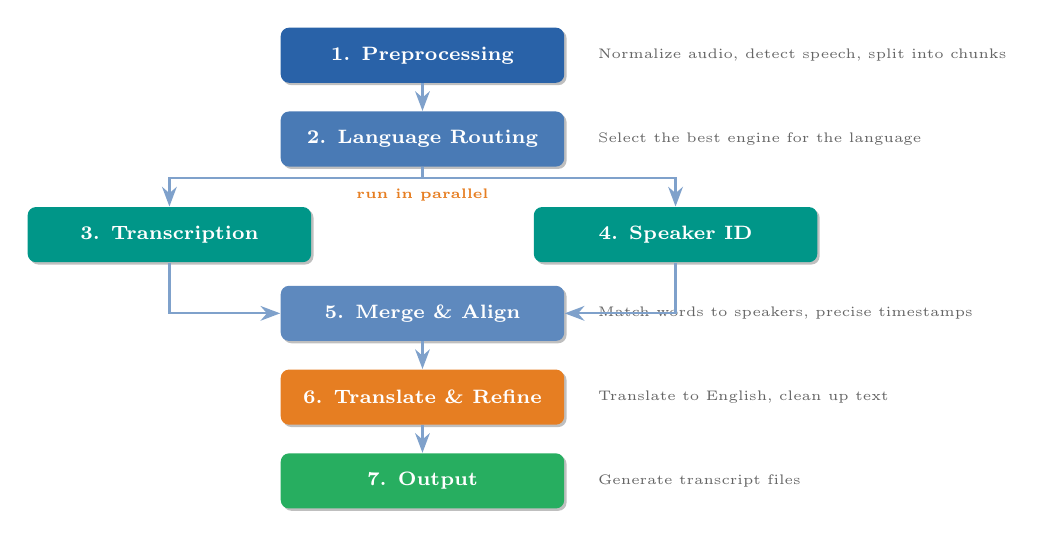
\begin{tikzpicture}[
        stage/.style={
            rounded corners=3pt,
            minimum width=3.6cm,
            minimum height=0.7cm,
            align=center,
            font=\scriptsize\bfseries,
            text=white,
            drop shadow={shadow xshift=0.3mm, shadow yshift=-0.3mm}
        },
        arr/.style={-{Stealth[length=2.5mm]}, thick, pipeblue!60},
        note/.style={font=\tiny, text=pipegray, align=left},
        scale=0.95
    ]
        % Stage 1
        \node[stage, fill=pipeblue] (s1) at (0, 0) {1. Preprocessing};
        \node[note, right=0.3cm of s1] {Normalize audio, detect speech, split into chunks};
        % Stage 2
        \node[stage, fill=pipeblue!85, below=0.35cm of s1] (s2) {2. Language Routing};
        \node[note, right=0.3cm of s2] {Select the best engine for the language};
        % Stages 3 & 4 (parallel)
        \node[stage, fill=pipeteal, below left=0.5cm and -0.4cm of s2] (s3) {3. Transcription};
        \node[stage, fill=pipeteal, below right=0.5cm and -0.4cm of s2] (s4) {4. Speaker ID};
        % Parallel bracket
        \node[font=\tiny\bfseries, text=pipeorange, below=0.15cm of s2] {run in parallel};
        % Stage 5
        \node[stage, fill=pipeblue!75, below=1.5cm of s2] (s5) {5. Merge \& Align};
        \node[note, right=0.3cm of s5] {Match words to speakers, precise timestamps};
        % Stage 6
        \node[stage, fill=pipeorange, below=0.35cm of s5] (s6) {6. Translate \& Refine};
        \node[note, right=0.3cm of s6] {Translate to English, clean up text};
        % Stage 7
        \node[stage, fill=pipegreen, below=0.35cm of s6] (s7) {7. Output};
        \node[note, right=0.3cm of s7] {Generate transcript files};
        % Arrows
        \draw[arr] (s1) -- (s2);
        \draw[arr] (s2.south) -- ++(0,-0.15) -| (s3.north);
        \draw[arr] (s2.south) -- ++(0,-0.15) -| (s4.north);
        \draw[arr] (s3.south) |- (s5.west);
        \draw[arr] (s4.south) |- (s5.east);
        \draw[arr] (s5) -- (s6);
        \draw[arr] (s6) -- (s7);
    \end{tikzpicture}
\end{frame}

% ============================================================================
\section{Stage Details}
% ============================================================================

% ── Slide 7: Preprocessing ────────────────────────────────────────────────
\begin{frame}{Stage 1: Audio Preprocessing}
    \begin{columns}[T]
        \begin{column}{0.48\textwidth}
            \begin{block}{What Happens}
                \scriptsize
                \begin{enumerate}
                    \item \textbf{Format conversion} --- any format to WAV (16\,kHz, mono)
                    \item \textbf{Loudness normalization} --- consistent volume (EBU R128)
                    \item \textbf{Noise reduction} --- spectral gating
                    \item \textbf{Voice detection} --- separates speech from silence/noise/music
                    \item \textbf{Chunking} --- splits long recordings into segments
                \end{enumerate}
            \end{block}
        \end{column}
        \begin{column}{0.48\textwidth}
            \begin{block}{Why It Matters}
                \scriptsize
                \begin{itemize}
                    \item Handles \textbf{any input format} (MP3, M4A, WAV, etc.)
                    \item Improves accuracy by \textbf{reducing noise}
                    \item \textbf{Audio quality metrics} in output (speech ratio, silence gaps)
                    \item Non-speech classified as \textbf{silence}, \textbf{noise}, or \textbf{music}
                \end{itemize}
            \end{block}
            \vspace{0.3em}
            \begin{exampleblock}{Tools Used}
                FFmpeg, Silero VAD, Spectral Gating
            \end{exampleblock}
        \end{column}
    \end{columns}
\end{frame}

% ── Slide 8: Language Routing ──────────────────────────────────────────────
\begin{frame}{Stage 2: Intelligent Language Routing}
    \centering
    \begin{tikzpicture}[
        tier/.style={
            rounded corners=5pt,
            minimum width=5.5cm,
            minimum height=2.2cm,
            align=center,
            text=white,
            font=\small,
            drop shadow
        },
        arr/.style={-{Stealth[length=3mm]}, very thick},
        scale=0.9
    ]
        % Input
        \node[rounded corners=3pt, fill=pipeblue, text=white, font=\small\bfseries,
              minimum width=3cm, minimum height=0.7cm] (input) at (0, 2) {Language Code};
        % High resource
        \node[tier, fill=pipeteal] (high) at (-4, -0.8) {
            \textbf{\large Whisper Large-v3}\\[4pt]
            \footnotesize 18 high-resource languages\\[2pt]
            \footnotesize English, Spanish, French, Arabic,\\[-1pt]
            \footnotesize Chinese, German, Portuguese \ldots\\[4pt]
            \footnotesize \faCheckCircle\ Highest accuracy
        };
        % Non-high resource
        \node[tier, fill=pipeorange] (nonhigh) at (4, -0.8) {
            \textbf{\large Omnilingual ASR}\\[4pt]
            \footnotesize 1,600+ languages\\[2pt]
            \footnotesize Hindi, Amharic, Swahili, Nepali,\\[-1pt]
            \footnotesize Burmese, Hausa, Yoruba \ldots\\[4pt]
            \footnotesize \faGlobeAfrica\ Broadest coverage
        };
        % Arrows
        \draw[arr, pipeteal] (input.south) -- ++(-0.3, -0.3) -| (high.north)
            node[midway, above left, font=\tiny\bfseries, text=pipeteal] {high-resource};
        \draw[arr, pipeorange] (input.south) -- ++(0.3, -0.3) -| (nonhigh.north)
            node[midway, above right, font=\tiny\bfseries, text=pipeorange] {other languages};
    \end{tikzpicture}
    \vspace{0.5em}
    \begin{block}{}
        \centering
        The pipeline automatically selects the \textbf{best-performing engine} for each language.\\
        Adding a new language requires \textbf{only one line of configuration}.
    \end{block}
\end{frame}

% ── Slide 9: Stages 3 & 4 ─────────────────────────────────────────────────
\begin{frame}{Stages 3 \& 4: Transcription + Speaker Identification}
    \begin{columns}[T]
        \begin{column}{0.48\textwidth}
            \begin{block}{\faMicrophone\ \ Stage 3: Transcription}
                \scriptsize
                \textbf{Converts speech to text}
                \vspace{0.2em}
                \begin{itemize}
                    \item \textbf{Whisper Large-v3} for high-resource languages
                        \begin{itemize}
                            \scriptsize
                            \item State-of-the-art accuracy
                            \item Word-level timestamps
                        \end{itemize}
                    \item \textbf{Omnilingual CTC 300M} for all others
                        \begin{itemize}
                            \scriptsize
                            \item Meta's multilingual model
                            \item Native code-switching support
                        \end{itemize}
                \end{itemize}
            \end{block}
        \end{column}
        \begin{column}{0.48\textwidth}
            \begin{block}{\faUsers\ \ Stage 4: Speaker Identification}
                \scriptsize
                \textbf{Detects who speaks when}
                \vspace{0.2em}
                \begin{itemize}
                    \item Auto-determines \textbf{number of speakers}
                    \item Labels: {\small\texttt{SPEAKER\_00}, \texttt{SPEAKER\_01}} \ldots
                    \item Works \textbf{independently} of language
                    \item Can override speaker count if known
                \end{itemize}
                \vspace{0.2em}
                \begin{exampleblock}{Two Backends}
                    \scriptsize
                    \textbf{pyannote 3.1} (default) or \textbf{NeMo MSDD} (overlap-aware)
                \end{exampleblock}
            \end{block}
        \end{column}
    \end{columns}
    \vspace{0.3em}
    \centering
    \colorbox{pipeorange!15}{\parbox{0.7\textwidth}{\centering
        \small\faRocket\ \ These two stages run \textbf{in parallel} on the GPU, saving significant processing time.
    }}
\end{frame}

% ── Slide 10: Alignment + Translation ─────────────────────────────────────
\begin{frame}{Stages 5--6: Alignment, Translation \& Refinement}
    \begin{columns}[T]
        \begin{column}{0.48\textwidth}
            \begin{block}{\faCrosshairs\ \ Stage 5: Merge \& Align}
                \scriptsize
                \begin{itemize}
                    \item Matches each \textbf{word to its speaker} via temporal overlap
                    \item \textbf{Forced alignment} (wav2vec2 MMS) refines timestamps
                    \item Whisper: $\pm$200ms--1s drift $\rightarrow$ after alignment: \textbf{$\sim$20ms}
                    \item Same-speaker segments \textbf{merged} into natural turns
                \end{itemize}
            \end{block}
        \end{column}
        \begin{column}{0.48\textwidth}
            \begin{block}{\faLanguage\ \ Stage 6: Translate \& Refine}
                \scriptsize
                \textbf{TranslateGemma 4B} (default):
                \begin{itemize}
                    \item Single model: translation + text cleanup
                    \item \textbf{4-bit quantized} $\rightarrow$ $\sim$2.5\,GB VRAM
                    \item 55 languages supported
                \end{itemize}
                \vspace{0.2em}
                \textbf{Alternative:} CT2 NLLB + Ollama LLM
                \begin{itemize}
                    \item NLLB-200 for translation (200+ languages)
                    \item LLM for refinement (Qwen 2.5:7b)
                \end{itemize}
            \end{block}
        \end{column}
    \end{columns}
    \vspace{0.2em}
    \centering
    \colorbox{pipeblue!10}{\parbox{0.85\textwidth}{\centering
        \scriptsize\faMemory\ \ ASR/diarization models are \textbf{fully unloaded} before translation loads --- peak VRAM stays within 6\,GB.
    }}
\end{frame}

% ── Slide 11: Output ──────────────────────────────────────────────────────
\begin{frame}[fragile]{Stage 7: Output}
    \begin{columns}[T]
        \begin{column}{0.52\textwidth}
            \begin{block}{Real Output --- Spanish Test (excerpt)}
                \begin{lstlisting}[basicstyle=\ttfamily\tiny, linewidth=\columnwidth]
======================================
TRANSCRIPT
======================================
Duration:    00:20:00
Languages:   Spanish
Speakers:    5 identified
ASR Engine:  Whisper large-v3
Audio:       61% speech | 39% non-speech
======================================
        [NOISE -- 7.2s]
[00:00:07] SPEAKER_00:
[es] Y como le he comentado,
     queremos comprender mejor los
     tipos de cuidado infantil...
[en] As I mentioned earlier, we want
     to better understand the types
     of childcare provided...
[00:00:20] SPEAKER_00:
[es] Si gusta les dejo la cartita
     de presentacion de la empresa.
[en] If you like, I will include the
     company introductory letter.
======================================
                \end{lstlisting}
            \end{block}
        \end{column}
        \begin{column}{0.44\textwidth}
            \begin{block}{Output Formats}
                \scriptsize
                \begin{itemize}
                    \item[\faFileAlt] \textbf{TXT} --- Research transcript with metadata
                    \item[\faCode] \textbf{JSON} --- Structured data for analysis
                    \item[\faClosedCaptioning] \textbf{SRT} --- Subtitles for video
                    \item[\faLayerGroup] \textbf{All} --- Generate all at once
                \end{itemize}
            \end{block}
            \vspace{0.2em}
            \begin{block}{Transcript Includes}
                \scriptsize
                \begin{itemize}
                    \item Full metadata header
                    \item Speaker labels per turn
                    \item Original text + English translation
                    \item Non-speech markers (silence, noise, music)
                    \item Audio quality metrics
                \end{itemize}
            \end{block}
        \end{column}
    \end{columns}
\end{frame}

% ============================================================================
\section{Language Extensibility}
% ============================================================================

% ── Slide 12: Language Coverage ────────────────────────────────────────────
\begin{frame}[fragile]{Language Coverage \& Adding New Languages}
    \begin{columns}[T]
        \begin{column}{0.32\textwidth}
            \begin{block}{\scriptsize High-Resource (Whisper)}
                \begin{multicols}{2}
                    \begin{itemize}
                        \tiny
                        \item English
                        \item Spanish
                        \item French
                        \item German
                        \item Portuguese
                        \item Russian
                        \item Chinese
                        \item Japanese
                        \item Korean
                        \item Italian
                        \item Dutch
                        \item Polish
                        \item Turkish
                        \item Czech
                        \item Swedish
                        \item Ukrainian
                        \item Romanian
                        \item Arabic
                    \end{itemize}
                \end{multicols}
            \end{block}
        \end{column}
        \begin{column}{0.32\textwidth}
            \begin{block}{\scriptsize Low-Resource (Omnilingual)}
                \begin{multicols}{2}
                    \begin{itemize}
                        \tiny
                        \item Hindi
                        \item Bengali
                        \item Nepali
                        \item Swahili
                        \item Amharic
                        \item Oromo
                        \item Hausa
                        \item Yoruba
                        \item Igbo
                        \item Tagalog
                        \item Burmese
                        \item Khmer
                        \item Kinyarwanda
                        \item Somali
                        \item Tigrinya
                        \item \textit{+ 1,585}
                    \end{itemize}
                \end{multicols}
            \end{block}
        \end{column}
        \begin{column}{0.33\textwidth}
            \begin{exampleblock}{\faPlus\ \ Add a Language}
                \scriptsize
                One YAML entry --- no retraining:
                \begin{lstlisting}[basicstyle=\ttfamily\tiny, frame=none, backgroundcolor=\color{lightbg}]
wol:
  name: "Wolof"
  tier: "non_high"
  bcp47: "wo"
  script: "Latn"
  nllb_code: "wol_Latn"
                \end{lstlisting}
            \end{exampleblock}
            \vspace{0.1em}
            \begin{alertblock}{\faExchangeAlt\ \ Code-Switching}
                \scriptsize
                Handles mid-sentence language switching automatically.
            \end{alertblock}
            \vspace{0.1em}
            \begin{block}{\faGlobeAmericas\ \ Zero-Shot}
                \scriptsize
                Unseen languages: auto-fallback to LLM variant.
            \end{block}
        \end{column}
    \end{columns}
\end{frame}

% ── Slide 13: Fine-Tuning ─────────────────────────────────────────────────
\begin{frame}[fragile]{Fine-Tuning for New Languages}
    \begin{columns}[T]
        \begin{column}{0.48\textwidth}
            \begin{block}{\faWrench\ \ Why Fine-Tune?}
                \scriptsize
                \begin{itemize}
                    \item Out-of-the-box: CER $<$10\% for \textbf{78\%} of 1,600+ languages
                    \item Fine-tuning pushes accuracy \textbf{significantly higher}
                    \item Useful for \textbf{dialectal variation} or \textbf{domain-specific} vocab
                \end{itemize}
            \end{block}
            \vspace{0.2em}
            \begin{exampleblock}{\faCheckCircle\ \ Straightforward Process}
                \scriptsize
                \begin{enumerate}
                    \item Prepare audio + transcription pairs
                    \item Use Meta's fine-tuning recipes (wav2vec2 CTC)
                    \item CTC 300M fits on a \textbf{single 6\,GB GPU}
                    \item Point pipeline config to new checkpoint
                \end{enumerate}
            \end{exampleblock}
        \end{column}
        \begin{column}{0.48\textwidth}
            \begin{block}{\faCode\ \ Pipeline Integration}
                \scriptsize
                \texttt{LanguageConfig} supports custom checkpoints:
                \begin{lstlisting}[basicstyle=\ttfamily\tiny, frame=none, backgroundcolor=\color{lightbg}]
class LanguageConfig:
    name: str
    tier: LanguageTier
    bcp47: str
    script: str
    nllb_code: str
    fine_tuned_checkpoint: Optional[str]
                \end{lstlisting}
                \vspace{0.2em}
                Register in YAML:
                \begin{lstlisting}[basicstyle=\ttfamily\tiny, frame=none, backgroundcolor=\color{lightbg}]
wol:
  name: "Wolof"
  tier: "non_high"
  fine_tuned_checkpoint:
    "./models/wolof_ctc300m.pt"
                \end{lstlisting}
                \vspace{0.1em}
                \scriptsize
                Recipes: \tiny\texttt{github.com/facebookresearch/omnilingual-asr}
            \end{block}
        \end{column}
    \end{columns}
\end{frame}

% ============================================================================
\section{Usage}
% ============================================================================

% ── Slide 14: How to Use It ───────────────────────────────────────────────
\begin{frame}[fragile]{How to Use It}
    \begin{block}{Basic Usage}
        \begin{lstlisting}[language=bash, basicstyle=\ttfamily\scriptsize]
# Transcribe a Spanish interview
asr-pipeline transcribe interview.mp3 --language spa
# Hindi focus group with 5 speakers, JSON output
asr-pipeline transcribe focus_group.wav --language hin \
    --max-speakers 5 --format json
# Amharic with project name
asr-pipeline transcribe meeting.m4a --language amh \
    --project "Ethiopia Study" --output-dir ./transcripts
        \end{lstlisting}
    \end{block}
    \vspace{-0.2em}
    \begin{columns}[T]
        \begin{column}{0.48\textwidth}
            \begin{exampleblock}{Other Commands}
                \scriptsize
                \texttt{list-languages} --- show languages\\
                \texttt{check-deps} --- verify install\\
                \texttt{setup} --- configure models
            \end{exampleblock}
        \end{column}
        \begin{column}{0.48\textwidth}
            \begin{exampleblock}{Configuration}
                \scriptsize
                All settings via \textbf{YAML config}: audio, engine selection, output format, hardware.
            \end{exampleblock}
        \end{column}
    \end{columns}
\end{frame}

% ============================================================================
\section{Next Steps}
% ============================================================================

% ── Slide 15: Next Steps & Roadmap ─────────────────────────────────────────
\begin{frame}{Next Steps}
    \begin{columns}[T]
        \begin{column}{0.48\textwidth}
            \begin{exampleblock}{\faCheckCircle\ \ Done}
                \scriptsize
                \begin{itemize}
                    \item Full 7-stage pipeline, end-to-end
                    \item 1,600+ language support
                    \item 8 min for 20 min audio on 6\,GB GPU
                    \item Speaker diarization (2 backends)
                    \item Translation + refinement
                    \item Multiple output formats (TXT, JSON, SRT)
                    \item Forced alignment for precise timestamps
                    \item Memory-efficient GPU management
                \end{itemize}
            \end{exampleblock}
            \vspace{0.2em}
            \begin{block}{\faLightbulb\ \ Future Possibilities}
                \scriptsize
                \begin{itemize}
                    \item Web interface for non-technical users
                    \item Real-time transcription mode
                    \item Custom vocabulary support
                \end{itemize}
            \end{block}
        \end{column}
        \begin{column}{0.48\textwidth}
            \begin{alertblock}{\faArrowRight\ \ Immediate Next Steps}
                \scriptsize
                \begin{enumerate}
                    \item \textbf{Single-file quality assessment}\\
                        {\scriptsize Run pipeline on one audio, review transcript accuracy, speaker assignment, translation quality.}
                    \vspace{0.2em}
                    \item \textbf{Batch processing (ZIP input)}\\
                        {\scriptsize Accept a \textbf{ZIP folder} of audio files, produce a folder of transcripts. Output files \textbf{match input filenames} for easy pairing with survey/para-data.}
                    \vspace{0.2em}
                    \item \textbf{Language-specific fine-tuning}\\
                        {\scriptsize Fine-tune CTC 300M on project languages to improve accuracy beyond baseline.}
                \end{enumerate}
            \end{alertblock}
        \end{column}
    \end{columns}
\end{frame}

% ── Thank You ───────────────────────────────────────────────────────────────
\begin{frame}[plain]
    \centering
    \vspace{2cm}
    {\Huge\bfseries\color{pipeblue} Thank You}

    \vspace{1cm}
    {\large\color{pipegray} Questions \& Discussion}

    \vspace{1.5cm}
    {\small\color{pipegray}
        \faTerminal\ \ \texttt{asr-pipeline transcribe audio.mp3 --language spa}
    }
\end{frame}

\end{document}
